\documentclass[a4paper,11pt,oneside]{memoir}

% Castellano
\usepackage[spanish,es-tabla]{babel}
\selectlanguage{spanish}
\usepackage[utf8]{inputenc}
\usepackage{placeins}

\RequirePackage{booktabs}
\RequirePackage[table]{xcolor}
\RequirePackage{xtab}
\RequirePackage{multirow}

% Links
\usepackage[colorlinks]{hyperref}
\hypersetup{
	allcolors = {red}
}

% Ecuaciones
\usepackage{amsmath}

% Rutas de fichero / paquete
\newcommand{\ruta}[1]{{\sffamily #1}}

% Párrafos
\nonzeroparskip


% Imagenes
\usepackage{graphicx}
\newcommand{\imagen}[2]{
	\begin{figure}[!h]
		\centering
		\includegraphics[width=0.9\textwidth]{#1}
		\caption{#2}\label{fig:#1}
	\end{figure}
	\FloatBarrier
}

\newcommand{\imagenflotante}[2]{
	\begin{figure}%[!h]
		\centering
		\includegraphics[width=0.9\textwidth]{#1}
		\caption{#2}\label{fig:#1}
	\end{figure}
}



% El comando \figura nos permite insertar figuras comodamente, y utilizando
% siempre el mismo formato. Los parametros son:
% 1 -> Porcentaje del ancho de página que ocupará la figura (de 0 a 1)
% 2 --> Fichero de la imagen
% 3 --> Texto a pie de imagen
% 4 --> Etiqueta (label) para referencias
% 5 --> Opciones que queramos pasarle al \includegraphics
% 6 --> Opciones de posicionamiento a pasarle a \begin{figure}
\newcommand{\figuraConPosicion}[6]{%
  \setlength{\anchoFloat}{#1\textwidth}%
  \addtolength{\anchoFloat}{-4\fboxsep}%
  \setlength{\anchoFigura}{\anchoFloat}%
  \begin{figure}[#6]
    \begin{center}%
      \Ovalbox{%
        \begin{minipage}{\anchoFloat}%
          \begin{center}%
            \includegraphics[width=\anchoFigura,#5]{#2}%
            \caption{#3}%
            \label{#4}%
          \end{center}%
        \end{minipage}
      }%
    \end{center}%
  \end{figure}%
}

%
% Comando para incluir imágenes en formato apaisado (sin marco).
\newcommand{\figuraApaisadaSinMarco}[5]{%
  \begin{figure}%
    \begin{center}%
    \includegraphics[angle=90,height=#1\textheight,#5]{#2}%
    \caption{#3}%
    \label{#4}%
    \end{center}%
  \end{figure}%
}
% Para las tablas
\newcommand{\otoprule}{\midrule [\heavyrulewidth]}
%
% Nuevo comando para tablas pequeñas (menos de una página).
\newcommand{\tablaSmall}[5]{%
 \begin{table}
  \begin{center}
   \rowcolors {2}{gray!35}{}
   \begin{tabular}{#2}
    \toprule
    #4
    \otoprule
    #5
    \bottomrule
   \end{tabular}
   \caption{#1}
   \label{tabla:#3}
  \end{center}
 \end{table}
}

%
% Nuevo comando para tablas pequeñas (menos de una página).
\newcommand{\tablaSmallSinColores}[5]{%
 \begin{table}[H]
  \begin{center}
   \begin{tabular}{#2}
    \toprule
    #4
    \otoprule
    #5
    \bottomrule
   \end{tabular}
   \caption{#1}
   \label{tabla:#3}
  \end{center}
 \end{table}
}

\newcommand{\tablaApaisadaSmall}[5]{%
\begin{landscape}
  \begin{table}
   \begin{center}
    \rowcolors {2}{gray!35}{}
    \begin{tabular}{#2}
     \toprule
     #4
     \otoprule
     #5
     \bottomrule
    \end{tabular}
    \caption{#1}
    \label{tabla:#3}
   \end{center}
  \end{table}
\end{landscape}
}

%
% Nuevo comando para tablas grandes con cabecera y filas alternas coloreadas en gris.
\newcommand{\tabla}[6]{%
  \begin{center}
    \tablefirsthead{
      \toprule
      #5
      \otoprule
    }
    \tablehead{
      \multicolumn{#3}{l}{\small\sl continúa desde la página anterior}\\
      \toprule
      #5
      \otoprule
    }
    \tabletail{
      \hline
      \multicolumn{#3}{r}{\small\sl continúa en la página siguiente}\\
    }
    \tablelasttail{
      \hline
    }
    \bottomcaption{#1}
    \rowcolors {2}{gray!35}{}
    \begin{xtabular}{#2}
      #6
      \bottomrule
    \end{xtabular}
    \label{tabla:#4}
  \end{center}
}

%
% Nuevo comando para tablas grandes con cabecera.
\newcommand{\tablaSinColores}[6]{%
  \begin{center}
    \tablefirsthead{
      \toprule
      #5
      \otoprule
    }
    \tablehead{
      \multicolumn{#3}{l}{\small\sl continúa desde la página anterior}\\
      \toprule
      #5
      \otoprule
    }
    \tabletail{
      \hline
      \multicolumn{#3}{r}{\small\sl continúa en la página siguiente}\\
    }
    \tablelasttail{
      \hline
    }
    \bottomcaption{#1}
    \begin{xtabular}{#2}
      #6
      \bottomrule
    \end{xtabular}
    \label{tabla:#4}
  \end{center}
}

%
% Nuevo comando para tablas grandes sin cabecera.
\newcommand{\tablaSinCabecera}[5]{%
  \begin{center}
    \tablefirsthead{
      \toprule
    }
    \tablehead{
      \multicolumn{#3}{l}{\small\sl continúa desde la página anterior}\\
      \hline
    }
    \tabletail{
      \hline
      \multicolumn{#3}{r}{\small\sl continúa en la página siguiente}\\
    }
    \tablelasttail{
      \hline
    }
    \bottomcaption{#1}
  \begin{xtabular}{#2}
    #5
   \bottomrule
  \end{xtabular}
  \label{tabla:#4}
  \end{center}
}



\definecolor{cgoLight}{HTML}{EEEEEE}
\definecolor{cgoExtralight}{HTML}{FFFFFF}

%
% Nuevo comando para tablas grandes sin cabecera.
\newcommand{\tablaSinCabeceraConBandas}[5]{%
  \begin{center}
    \tablefirsthead{
      \toprule
    }
    \tablehead{
      \multicolumn{#3}{l}{\small\sl continúa desde la página anterior}\\
      \hline
    }
    \tabletail{
      \hline
      \multicolumn{#3}{r}{\small\sl continúa en la página siguiente}\\
    }
    \tablelasttail{
      \hline
    }
    \bottomcaption{#1}
    \rowcolors[]{1}{cgoExtralight}{cgoLight}

  \begin{xtabular}{#2}
    #5
   \bottomrule
  \end{xtabular}
  \label{tabla:#4}
  \end{center}
}


















\graphicspath{ {./img/} }

% Capítulos
\chapterstyle{bianchi}
\newcommand{\capitulo}[2]{
	\setcounter{chapter}{#1}
	\setcounter{section}{0}
	\chapter*{#2}
	\addcontentsline{toc}{chapter}{#2}
	\markboth{#2}{#2}
}

% Apéndices
\renewcommand{\appendixname}{Apéndice}
\renewcommand*\cftappendixname{\appendixname}

\newcommand{\apendice}[1]{
	%\renewcommand{\thechapter}{A}
	\chapter{#1}
}

\renewcommand*\cftappendixname{\appendixname\ }

% Formato de portada
\makeatletter
\usepackage{xcolor}
\newcommand{\tutor}[1]{\def\@tutor{#1}}
\newcommand{\course}[1]{\def\@course{#1}}
\definecolor{cpardoBox}{HTML}{E6E6FF}
\def\maketitle{
  \null
  \thispagestyle{empty}
  % Cabecera ----------------
\noindent
\includegraphics[width=\textwidth]{cabecera}\vspace{1cm}%
  \vfill
  % Título proyecto y escudo informática ----------------
  \colorbox{cpardoBox}{%
    \begin{minipage}{.8\textwidth}
      \vspace{.5cm}\Large
      \begin{center}
      \textbf{TFG del Grado en Ingeniería Informática}\vspace{.6cm}\\
      \textbf{\LARGE\@title{}}
      \end{center}
      \vspace{.2cm}
    \end{minipage}

  }%
  \hfill\begin{minipage}{.20\textwidth}
    
\includegraphics[width=\textwidth]{escudoInfor}
  \end{minipage}
  \vfill
  % Datos de alumno, curso y tutores ------------------
  \begin{center}%
  {%
    \noindent\LARGE
    Presentado por \@author{}\\ 
    en Universidad de Burgos --- \@date{}\\
    Tutor: \@tutor{}\\
  }%
  \end{center}%
  \null
  \cleardoublepage
  }
\makeatother

\newcommand{\nombre}{Eduardo Tubilleja Calvo} %%% cambio de comando

% Datos de portada
\title{Ensembles de clasificadores multi-label en Scikit-Learn}
\author{\nombre}
\tutor{Dr. Álvar Arnaiz González\\y Dr. Juan José Rodríguez Díez}
\date{\today}

\begin{document}

\maketitle


\newpage\null\thispagestyle{empty}\newpage


%%%%%%%%%%%%%%%%%%%%%%%%%%%%%%%%%%%%%%%%%%%%%%%%%%%%%%%%%%%%%%%%%%%%%%%%%%%%%%%%%%%%%%%%
\thispagestyle{empty}


\noindent
\includegraphics[width=\textwidth]{cabecera}\vspace{1cm}

\noindent D. Álvar Arnaiz González y D. Juan José Rodríguez Díez, profesores del departamento de nombre departamento de Ingeniería Civil, área de Lenguajes y Sistemas Informáticos.

\noindent Exponen:

\noindent Que el alumno D. \nombre, con DNI 71298897R, ha realizado el Trabajo final de Grado en Ingeniería Informática titulado <<Ensembles de clasificadores multi-label en Scikit-Learn>>. 

\noindent Y que dicho trabajo ha sido realizado por el alumno bajo la dirección del que suscribe, en virtud de lo cual se autoriza su presentación y defensa.

\begin{center} %\large
En Burgos, {\large \today}
\end{center}

\vfill\vfill\vfill

% Author and supervisor
\begin{minipage}{0.45\textwidth}
\begin{flushleft} %\large
Vº. Bº. del Tutor:\\[2cm]
D. Álvar Arnaiz González
\end{flushleft}
\end{minipage}
\hfill
\begin{minipage}{0.45\textwidth}
\begin{flushleft} %\large
Vº. Bº. del Tutor:\\[2cm]
D. Juan José Rodríguez Díez
\end{flushleft}
\end{minipage}
\hfill

\vfill

% para casos con solo un tutor comentar lo anterior
% y descomentar lo siguiente
%Vº. Bº. del Tutor:\\[2cm]
%D. nombre tutor


\newpage\null\thispagestyle{empty}\newpage




\frontmatter

% Abstract en castellano
\renewcommand*\abstractname{Resumen}
\begin{abstract}
En este primer apartado se hace una \textbf{breve} presentación del tema que se aborda en el proyecto.
\end{abstract}

\renewcommand*\abstractname{Descriptores}
\begin{abstract}
Palabras separadas por comas que identifiquen el contenido del proyecto Ej: servidor web, buscador de vuelos, android \ldots
\end{abstract}

\clearpage

% Abstract en inglés
\renewcommand*\abstractname{Abstract}
\begin{abstract}
A \textbf{brief} presentation of the topic addressed in the project.
\end{abstract}

\renewcommand*\abstractname{Keywords}
\begin{abstract}
keywords separated by commas.
\end{abstract}

\clearpage

% Indices
\tableofcontents

\clearpage

\listoffigures

\clearpage

\listoftables
\clearpage

\mainmatter
\capitulo{1}{Introducción}

La minería de datos es un campo de 	las ciencias de la computación, que consisten en el análisis de grandes cantidades de datos para descubrir patrones.
Para ello se puede utilizar el aprendizaje automático, éste pertenece a un subcampo de las ciencias de computación y de la rama de inteligencia artificial, el objetivo del aprendizaje automático es desarrollar unas técnicas que permitan que las máquinas aprendan~\cite{wiki:datamining}.
Dentro de este aprendizaje se encuentra el aprendizaje supervisado, en él normalmente los conjuntos de datos suelen tener solo una variable a predecir, conocido como Single-Label, pero apareció el concepto de Multi-Label~\cite{multilabel2}, este hace referencia a los conjuntos de datos en lo que cada elemento de la base de datos puede pertenecer a más de una clase, como por ejemplo en el etiquetado de imágenes: en el que una imagen puede tener a la vez las etiquetas <<árbol>>, <<montaña>> y <<mar>>.

En este proyecto vamos a tratar de implementar diversos algoritmos de multi-clasificadores (\textit{ensembles}), para Multi-Label sobre la biblioteca de Python~\cite{python} Scikit-Learn~\cite{scikitlearn}. Se ha seguido la guía de estilo de Python (PeP~\cite{pep}) y las convecciones que se han observado en Sklearn (Scikit-Learn). Para que se entienda mejor y sea más gráfico, se han dibujado árboles y gráficas, mostrando los resultados al ejecutar dichos algoritmos sobre unos conjuntos de datos. Los algoritmos en los que nos vamos a centrar son Disturbing Neighbors~\cite{disturbingneighbors}, Random Oracles~\cite{randomoracles} y Rotation Forest~\cite{rotationforest}.

A lo largo del proyecto también veremos como funcionan los \textit{ensembles}.
Los métodos de \textit{ensembles} combinan las predicciones de unos clasificadores base, que están construidos mediante un algoritmo de aprendizaje para mejorar la solidez de si sólo tendríamos un clasificador~\cite{ensemble}.
El éxito de un \textit{ensemble} requiere que un clasificador base tenga exactitud y diversidad.
La ventaja de usar un \textit{ensemble} de clasificadores base consiste en la posibilidad que algunos de ellos pueden corregir una predicción incorrecta de otros, por lo que cuantos más clasificadores tengamos mas precisas serán las predicciones. 
¿Cómo puede un \textit{ensemble} de clasificadores base que han sido generados por el mismo algoritmo tener distintas salidas? Una de las estrategias que podemos usar para ello son los \textit{ensembles} homogéneos, es decir, mismo algoritmo entrenado con distinto conjunto de datos.

\capitulo{2}{Objetivos del proyecto}
Los objetivos del proyectos son:

\begin{enumerate}
\item Implementar un algoritmo en scikit-learn que .
\end{enumerate}

En el proyecto se implementarán los algoritmos que hemos considerado más interesantes, en el futuro se podrán ir añadiendo mas algoritmos.

\capitulo{3}{Conceptos teóricos}

Este apartado va a explicar los conceptos teóricos necesarios para poder entender el proyecto.

\section{Minería de Datos}
\begin{quote}
Es conocida la frase <<los datos en bruto raramente son beneficiosos directamente>>. Pueden tener valor, ya que podemos extraer información útil para la toma de decisiones o exploración, y también para la compresión del fenómeno dominante en el conjunto de datos~\cite{mineria}.
\end{quote}

La finalidad de esto es descubrir unos patrones, una similitud o una propensión que expliquen el comportamiento de los datos. Para hacer esto utiliza los métodos de la inteligencia artificial y estadística.
El objetivo del proceso de minería de datos consiste en extraer información de un conjunto de datos, luego se interpreta esta información para un uso posterior~\cite{wiki:datamining}.

La minería de datos está basada en el aprendizaje automático, para ello se considera un conjunto con $n$ muestras y se intenta predecir las propiedades de los datos desconocidos. Podemos separar los problemas de aprendizaje principalmente en dos~\cite{scikitlearn2}:
	\begin{itemize}
		\item Aprendizaje supervisado: Consiste en que a partir de un conjunto de datos, hacer predicciones basadas en el comportamiento o las características de dichos datos. Nos permite buscar patrones en datos. Dos de las tareas más comunes del aprendizaje supervisado son la clasificación y la regresión:
		
		\begin{itemize}
		 	\item Clasificación: El programa debe aprender a predecir en que categoría o clase irán los nuevos datos, según las nuevas observaciones, por ejemplo, predecir si el precio de una acción bajará o subirá.
		 	\item Regresión: El programa debe predecir el valor de una variable de respuesta continua, por ejemplo, predecir las ventas de un nuevo producto.
		\end{itemize}
		
		\item Aprendizaje no supervisado: Usa datos que no están etiquetados. El objetivo es explorarlos para encontrar alguna forma de organizarlos.
	\end{itemize}

La minería de datos está incluida en el proceso de KDD (Knowledge Discovery in Databases, Descubrimiento del conocimiento en bases de datos) Este proceso tiene una secuencia de pasos~\cite{mineria_KDD}:

\begin{enumerate}[1.]
	\item Limpieza de datos. Eliminación del ruido y la inconsistencia de los datos.
	\item Integración de los datos. Múltiples fuentes de datos son combinadas.
	\item Selección de datos. Los datos relevantes para la tarea de análisis se recuperan de la base de datos.
	\item Transformación de datos. Los datos son transformados y se consolidan como apropiados para la minería mediante la realización de operaciones simétricas o de agregación.
	\item Minería de datos. Es un proceso esencial donde los métodos de inteligencia son aplicados a la extracción de patrones.
	\item Evaluación de patrones. Identificar los patrones que de verdad son interesantes, que representan el conocimiento basado en medidas de interés.
	\item Presentación del conocimiento. Representación visual de los resultados obtenidos.
\end{enumerate}

Aunque el proceso de la minería de datos consta de más etapas nosotros nos centraremos en 4 etapas~\cite{datamining}:
\begin{itemize}
	\item Determinación de los objetivos: Se tratan los objetivos que quiere conseguir el cliente bajo un asesor especialista en minería de datos.
	\item Preprocesamiento de los datos: Es la etapa que más tiempo se tarda en realizar el proceso. Se seleccionan, limpian, enriquecen, reducen y transforman las bases de datos.
	\item Determinación del modelo: Se lleva a cabo un estudio estadístico de los datos, más tarde se hace una visualización gráfica para una primera aproximación. Según los objetivos que se habían propuesto se pueden usar diferentes algoritmos de la Inteligencia Artificial.
	\item  Análisis de los resultados: Se comprueban si los datos obtenidos tienen coherencia, después se comparan con los obtenidos en los estudios estadísticos y la visualización gráfica. El cliente es el que ve si los datos le aportan nuevo conocimiento que le permita considerar sus decisiones.
\end{itemize}

\section{Multi-Label}
Al principio el aprendizaje supervisado trataba con el análisis de datos de Single-Label donde los ejemplos de entrenamiento son asociados con un Single-Label de un conjunto que no tiene nada en común con otros conjuntos. Sin embargo, los ejemplos de entrenamiento a veces se pueden asociar a un conjunto de labels, a los que llamaremos Multi-Label~\cite{multilabel2}.

La clasificación Single-Label y Multi-Label son unas tareas que se pueden resolver con distintas técnicas de minería de datos, la cual nos permite que a partir de un conjunto de instancias de entrenamiento, podamos determinar a través de unos atributos esenciales de dichas instancias, crear unas reglas que posteriormente se usarán para clasificar nuevas instancias~\cite{multilabel}. Como por ejemplo en el etiquetado de imágenes: en el que una imagen puede tener a la vez las etiquetas <<árbol>>, <<montaña>> y <<mar>>.   

\section{\textit{Ensemble}}
Un \textit{ensemble} es un esquema de combinación de clasificadores base con los que obtenemos unas predicciones individuales. El éxito de un \textit{ensemble} requiere tanto exactitud como diversidad de sus clasificadores base. La diversidad representa como de diferente son las predicciones de los clasificadores base. Si los clasificadores base siempre están de acuerdo no habría diferencia entre usar sólo un clasificador base o varios combinado por un método de \textit{ensemble}. Entonces la ventaja de usar un \textit{ensemble} de clasificadores base consiste en la posibilidad que algunos de ellos pueden corregir una predicción incorrecta de otros, por lo que cuantos más clasificadores tengamos más precisas serán las predicciones. 

Es normal obtener estos clasificadores base en un \textit{ensemble} usando el mismo algoritmo, así que en esta situación el proceso de entrenamiento realizado por el \textit{ensemble} es la principal fuente de diversidad. La diversidad de Bagging~\cite{bagging} proviene de elegir al azar diferentes instancias para entrenar a cada clasificador de base. El método Random Subspaces~\cite{randomsubspace} elige diferentes subconjuntos de atributos para entrenar a cada clasificador base. Boosting~\cite{boosting} entrena de forma iterativa el conjunto de clasificadores base, modificando los pesos de las instancias para entrenar al clasificador actual. Estos nuevos pesos se calculan a partir del error de entrenamiento en el clasificador base anterior, por lo que cada nuevo clasificador de base llega más especializado en instancias que han sido mal clasificados antes. A veces los clasificadores base son muy estables y el  algoritmo de entrenamiento del \textit{ensemble} no es suficiente para proporcionar el nivel deseado de diversidad~\cite{disturbingneighbors}.

Los métodos de \textit{ensembles} combinan las predicciones de unos estimadores base, que están construidos mediante un algoritmo de aprendizaje para mejorar la solidez de un solo estimador~\cite{ensemble}.
Se distinguen dos clases de métodos de \textit{ensembles}:
	\begin{itemize}
		\item En los métodos de Bagging~\cite{bagging}, se construyen varios estimadores de forma independiente y luego se calcula su promedio para las predicciones.
		\item En los métodos de Boosting~\cite{boosting}, se construyen los estimadores secuencialmente y se trata de reducir el sesgo del estimador combinado. 
	\end{itemize}
	
Podemos ver un ejemplo de un ensemble de clasificadores en la siguiente figura~\ref{fig:Ensembles}~\cite{figensemble}.

\begin{figure}
\centering
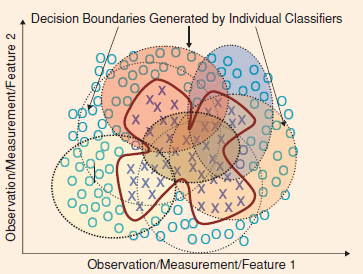
\includegraphics[width=0.95\textwidth]{Ensembles}
\caption{Ensemble de clasificadores que abarca un espacio de decisión}
\label{fig:Ensembles}
\end{figure}

\section{Disturbing Neighbors}

Los Disturbing Neighbors (DN) o vecinos molestones se han utilizado con éxito para mejorar la diversidad en los bosques~\cite{disturbingneighbors}.

El método DN trabaja en cada clasificador base de la siguiente manera:
\begin{itemize}
    \item $m$ instancias son seleccionadas aleatoriamente de el conjunto de datos de entrenamiento para construir un clasificador 1-NN. El valor $m$ suelen ser valores muy pequeños.
    \item Las dimensiones para calcular la distancia euclidea en el clasificador 1-NN, también se seleccionan. Como mínimo se seleccionan el 50\% de los atributos.
    \item Luego $m+1$ nuevas características son añadidas al conjunto de entrenamiento. Una de las características adicionales es la clase predicha por el clasificador 1-NN para cada instancia \textbf{x}, y las otras $m$ son características booleanas, todos los valores falsos excepto uno corresponden al vecino más cercano para esa instancia.
    \item El clasificador base está entrenado usando las características originales mas las nuevas $m+1$ características. 
\end{itemize}
Por lo tanto, el proceso normal de entrenamiento de los clasificadores base se altera añadiendo estas nuevas características del clasificador 1-NN. Es por eso que el método se llama vecinos molestones. La aleatoriedad aumenta la diversidad y se debe a:
\begin{itemize}
\item Los vecinos utilizados en cada clasificador 1-NN se seleccionan aleatoriamente. Por lo tanto, sus predicciones y las características booleanas son diferentes para cada clasificador base.
\item Las dimensiones utilizadas para calcular las distancias euclidianas también se eligen de forma aleatoria, así que si dos clasificadores básicos tienen al menos los mismos m vecinos, las predicciones 1-NN y las características booleanas podrían ser diferentes.
\end{itemize}

En resumen, Disturbing Neighbors es un método para alterar el proceso de entrenamiento normal de los clasificadores base en un \textit{ensemble}, mejorando su diversidad y mejorando la precisión general del \textit{ensemble}.

\section{Random Oracles}

Random Oracles son mini-ensembles formados por dos o más modelos, pueden usarse como modelos base para otros métodos \textit{ensemble}. El objetivo de usar Random Oracles es tener más diversidad entre los modelos base que forman un \textit{ensemble}~\cite{randomoracles}.

Dado un método base, el entrenamiento de un Random Oracle consiste en:
\begin{itemize}

	\item Seleccionar aleatoriamente un Random Oracle.
	\item Dividir los datos de entrenamiento en dos o más subconjuntos usando el Random Oracle.
	\item Para cada subconjunto de datos de entrenamiento, se construye un modelo (en nuestro caso un árbol, aunque se pueden construir otros modelos). El modelo Random Oracle está formado por los modelos cada subconjunto y el propio oráculo.
\end{itemize}
La predicción del test de una instancia se realiza de la siguiente manera: 
\begin{itemize}
	\item Usa el Random Oracle para seleccionar uno de los dos o más modelos.
	\item Devuelve la predicción obtenida por el modelo seleccionado.
\end{itemize}

Se pueden considerar diferentes tipos de Oracles. En este trabajo, se utiliza el Linear Random Oracle. Este oráculo divide el espacio en dos o más subespacios utilizando un hiperplano. Para construir el oráculo, dos o más objetos de entrenamiento diferentes se seleccionan aleatoriamente, cada objeto de entrenamiento restante se asigna al subespacio del objeto de entrenamiento seleccionado que está más cerca.

\section{Rotation Forest}

Rotation Forest, tiene como objetivo construir clasificadores precisos y diversos. La heurística principal consiste en aplicar la extracción de características a subconjuntos de características y reconstruir un conjunto completo de características para cada clasificador en el conjunto. En el artículo original se utiliza el Análisis de Componentes Principales (PCA)~\cite{rotationforest}.

Para construir el clasificador se siguen los siguientes pasos:
\begin{itemize}
	\item Dividir los atributos del conjunto de datos en $K$ subconjuntos. Para maximizar la diversidad se eligen subconjuntos disjuntos.
	\item De las clases se seleccionan las que son distintas, y de estas se selecciona una muestra, en nuestro caso la muestra tiene un tamaño del 80\%.
	\item Para cada subconjunto se selecciona aleatoriamente una muestra, por defecto con un tamaño del 75\%. Se ejecuta PCA sobre cada una de las muestras.
	\item Después de todos los pasos anteriores, para predecir se hace el \texttt{predict} del estimador base.
\end{itemize}

De esta forma, se construyen clasificadores individuales precisos.
\capitulo{4}{Técnicas y herramientas}

En este apartado de la memoria se presentan las técnicas metodológicas y las herramientas de desarrollo que se han utilizado para llevar a cabo el proyecto. 

%\maketitle
\section{GitHub}
Es una plataforma para alojar proyectos y utiliza git como sistema de control de versiones. Se organiza por tareas (milestones e issues).
Utiliza el framework Ruby on Rails~\cite{github}.

Podemos acceder a través de: \url{https://github.com/}

\textbf{Ventajas:}

\begin{itemize}
\item Es uno de los repositorios mas usados, por lo que es fácil encontrar información en Internet para resolver cualquier duda.

\item El código es público por lo que cualquiera puede proponer cambios en el mismo, seguirte y ver el proyecto.

\item Las distintas versiones del código están alojadas en la nube por lo que si perdemos el contenido de nuestro ordenador, podremos recuperarlo.
\end{itemize}

\textbf{Desventajas:}

\begin{itemize}
\item También puedes tener proyectos privados pero para ello tienes que utilizar una cuenta de pago, aunque los estudiantes e investigadores pueden obtener esto gratuitamente.
\end{itemize}

\section{Python}
Python es un lenguaje de programación interpretado se hace hincapié en que una sintaxis que favorezca un código legible~\cite{python}.
Se trata de un lenguaje de programación multiparadigma (permite crear programas utilizando mas de un estilo de programación), ya que soporta orientación a objetos, programación imperativa y programación funcional. Es un lenguaje interpretado, usa tipado dinámico (una variable puede tomar valores de distinto tipo) y es multiplataforma~\cite{wiki:python}.

Python es recomendable para programadores que empiezan por primera vez, o que vienen de ostros lenguajes, ya que hay mucha documentación para dar el primer paso en este lenguaje. La comunidad organiza conferencias y también colabora con el código.

Contiene miles de módulos de terceros, a parte de la biblioteca estándar de Python, por lo que tenemos infinitas posibilidades.

Por último, Python se desarrolla bajo una licencia de código abierto aprobada por OSI, por lo que es se puede utilizar libremente y distribuir. La licencia de Python es administrada por la Python Software Foundation. 

Podemos acceder a través de: 
\url{https://www.python.org/}

\section{Spyder}
Es un entorno de desarrollo interactivo para el lenguaje de Python, es de código abierto.
Tiene funciones avanzadas de edición, pruebas interactivas, depuración e introspección. También es un entorno informático numérico y tiene diversas bibliotecas que podemos utilizar, como pueden ser numpy~\cite{spyder}.

Podemos acceder a través de: 
\url{http://pythonhosted.org/spyder/}

\section{\LaTeX}
Se usa para la creación de documentos que necesiten una alta calidad tipográfica, como puede ser en artículos o libros científicos~\cite{latex}.

Podemos acceder a través de: 
\url{https://www.latex-project.org/}

\textbf{Ventajas:}
\begin{itemize}
\item Es software libre, por lo que no requiere ningún coste.
\item No te tienes preocupar por el diseño, ya que la herramienta se encarga de ello.
\end{itemize}

\textbf{Desventajas:}
\begin{itemize}
\item Si eres principiante necesitas un tiempo de aprendizaje para saber como funciona.
\end{itemize}

\section{Jupyter Notebook}
Es una aplicación web de código abierto, con él podemos crear y compartir documentos, que nos permiten visualizar los resultados al ejecutar nuestro código, ya sean imágenes, árboles..., que otros entornos de desarrollo (como Spyder mencionado anteriormente) no nos permiten esto.
Soporta más lenguajes, pero nosotros lo usaremos para el lenguaje de Python~\cite{jupyter}.

Podemos acceder a través de: 
\url{http://jupyter.org/}	

\section{Scikit-learn}
Es una librería de Python que contiene algoritmos de aprendizaje automático para problemas supervisados y no supervisados. Como esta basado en Python, puede integrarse fácilmente en aplicaciones que no suelen usarse para análisis de datos estdísticos. EL trabajo futuro incluye aprendizaje en línea para escalar a grandes conjuntos de datos~\cite{scikitlearn}. 

Podemos acceder a través de: 
\url{http://scikit-learn.org/stable/}

\section{SonarQube}
Es una plataforma que sirve para evaluar y analizar código. Es software libre, para llevar a cabo este análisis del código utiliza distintas herramientas como pueden ser Checkstyle, PMD o FindBugs, con dichas herramientas obtenemos métricas que nos ayudan a mejorar la calidad de nuestro código fuente~\cite{wiki:sonarqube}.

Los aspectos que evalúa esta herramienta son:
\begin{itemize}
	\item Technical Debt, esta parte nos indica los aspectos y métricas que no habíamos tenido en cuenta y también nos muestran la claridad del código. Una de las ventajas es que te indica donde has cometido una falta de estilo o donde tienes demasiada complejidad.
	\item La complejidad, los cambios de flujo que sufre el código, es decir, las condiciones if, while for… 
	\item Podemos ver las líneas de código que hemos escrito en cada fichero (sin contar los comentarios).
	\item Si queremos evaluar más aspectos, podemos instalar Plugins que nos lo permiten.
\end{itemize}

Podemos acceder a través de: 
\url{https://www.sonarqube.org/}

\section{Graphviz}
Es un software de visualización gráfica de código abierto. Es una forma de representar nuestra información estructural como diagramas de gráficos y redes abstractas. En nuestro caso lo utilizamos para dibujar un  árbol de nuestro conjunto de datos entrenado. Su arquitectura consiste en un lenguaje de descripción de gráficos llamado DOT.

Podemos acceder a través de: 
\url{https://www.graphviz.org/}

\section{Zenhub}
Es un gestor de tareas es similiar a Trello \url{https://trello.com/}, tiene un modo pizarra en el que podemos ver los cambios. Una de las grandes ventajas es que podemos integrarlo desde GitHub, por lo que no es necesario el uso de una aplicación externa. Una pequeña desventaja podríamos decir que es que no se puede añadir código, pero como el repositorio de GitHub nos permite visualizar dicho código no es un gran problema.

Podemos acceder a través de: 
\url{https://www.zenhub.com/}
\capitulo{5}{Aspectos relevantes del desarrollo del proyecto}

\section{Formación}
El proyecto requería unos conocimientos técnicos de los que desconocía en un principio. Entre ellos, conocimientos sobre Minería de datos, Scikit-Learn y documentar en \LaTeX. Para aprender estos conocimientos se ha necesitado leer documentos científicos, descubriendo la utilidad de ellos, ya que nunca había hecho uso de ellos.

Fue necesario instruirse en cómo implementar algoritmos, para ello tomamos de ejemplo, los algoritmos ya implementados en Scikit-Learn.

Otro de los conocimientos adquiridos en la realización de ese proyecto ha sido la librería Scikit-Learn, porque nosotros queremos implementar algoritmos en dicha librería, porque vamos a tratar la minería de datos, y como queremos clasificar un conjunto de datos para después de entrar poder predecir unos resultados con la mayor precisión posible, Sickit-Learn es una librería perfecta para esto. 

\section{Calidad del Software}
Cualquier persona con pocos conocimientos en minería de datos o programación en Python, puede usarla ya que se han generado unos notebooks para ello, por lo que podremos ejecutarlos teniendo mínimos conocimientos en el tema.

Se ha conseguido una buena calidad de código, ya que se ha comprobado en SonarQube, y tenemos la mejor nota posible. Para tener código claro y fácil de entender se ha ido comentado los métodos/funciones para ver lo que hacer cada parte del código. Se ha seguido la guía de estilo de Python y Pep~\cite{pep}.

Se han realizado unos análisis con distintas medidas y distintos conjuntos de datos para cada uno de los algoritmos creados. Después de esto hemos podido ver que el algoritmo Rotation Forest, es mejor que los otros dos algoritmos, aunque Random Oracle le sigue muy de cerca, ya que en las distintas medidas que se han comprobado los resultados eran solo un poco peores. Respecto a Disturbing Neighbors, es el peor de los tres, ya que este si hay una diferencia notable en los resultados, respecto a los otros dos. Esto no quiere decir que siempre Distutbing Neighbors vaya ser peor, ya que se ha probado solo para algunos conjuntos de datos.
\capitulo{6}{Trabajos relacionados}
En este apartado vamos a analizar y comparar nuestro proyecto con otros relacionados. Lo dividiremos en tres partes, una en la que hablaremos de otras librerías ensembles, otra parte sobre librerías de aprendizaje automático y una última de servicios de computación en la nube.

\section{Librerías con implementaciones de \textit{ensembles}}
A parte de de la librería que hemos usado de Scikit-Learn, existen librerías similares. A continuación, analizaremos algunas de ellas.

\subsection{EnsembleSVM}
Esta biblioteca de aprendizaje automático es de software libre. Esta librería nos ofrece la funcionalidad para llevar a cabo el aprendizaje de ensembles utilizando modelos base de la máquina de vectores de soporte (SVM). Permite entrenar eficientemente modelos para grandes conjuntos de datos~\cite{ensembleSVM}.

\subsection{$H_2O$ \textit{Ensemble}}
Es una librería de R, que nos proporciona funcionalidad para crear conjuntos a partir de algoritmos básicos de aprendizaje que podemos acceder a través de este paquete. Este tipo de aprendizaje de ensembles se conoce como <<súper aprendizaje>>. Este algoritmos aprende de la combinación óptima de los entrenamientos~\cite{ensembleh2o}.

\section{Librerías de aprendizaje automático Single-Label}
Vamos a ver diferentes librerías de aprendizaje automático para Single-Label.
\subsection{Weka}
Es una colección de algoritmos de aprendizaje automático para tareas de minería de datos. Los algoritmos se pueden aplicar sobre un conjunto de datos o llamar desde su propio código de java. Contiene herramientas para el preprocesamiento de datos, clasificación, clustering, reglas de asociación y visualización. Es un software de código abierto con la licencia de GNU~\cite{weka}. 

\subsection{Keel}
Es una herramienta de software de código abierto de Java, que se puede utilizar para una gran cantidad de tareas de descubrimiento de datos de conocimiento diferentes. Proporciona una GUI simple basada en el flujo de datos para diseñar experimentos con diferentes conjuntos de datos y algoritmos de inteligencia computacional, con el fin de evaluar el comportamiento de los algoritmos. Contiene una amplia variedad de algoritmos clásicos de extracción de conocimiento, técnicas de preprocesamiento, algoritmos de aprendizaje basados en inteligencia computacional, modelos híbridos...

Permite realizar un análisis completo de nuevas propuestas de inteligencia computacional en comparación con las existentes~\cite{keel}.

\subsection{TensorFlow}
Es una librería de computación numérica que computa gradientes automáticamente. Es un sistema flexible y se puede utilizar para gran variedad de algoritmos, incluidos de entrenamiento e inferencia para modelos de redes neuronales. Se ha utilizado para realizar investigaciones y para implementar sistemas de aprendizaje automático en diferentes áreas~\cite{tensorflow}.

Ha sido desarrollada por Google, y la utilizan empresas como Dropbox, Uber y Snapchat~\cite{libraries}.

\subsection{Pytorch}
Es una biblioteca de aprendizaje de máquina de código abierto para Python que permite un crecimiento rápido de Deep Learning. Su mayor característica es que utiliza grafos computacionales dinámicos.

Ha sido desarrollado principalmente por el grupo de investigación de inteligencia artificial de Facebook, y por ejemplo el software <<Pyro>> de Uber para la programación probabilística se basa en él~\cite{wiki:pytorch}.

\section{Librerías de aprendizaje automático Multi-Label}
Vamos a ver diferentes librerías de aprendizaje automático para Multi-Label.
\subsection{Meka}
Proporciona una implementación de código abierto de métodos para aprendizaje y evaluación de Multi-Label. En la clasificación Multi-Label, queremos predecir múltiples variables de salida para cada instancia de entrada. Esto es diferente del caso estándar que involucra solo una única variable objetivo. MEKA se basa en Weka, incluye docenas de métodos Multi-Label de la literatura científica, y esta relacionado con el framework de MULAN~\cite{meka}.

\subsection{Mulan}
Es una biblioteca de código abierto de Java para aprender de conjuntos de datos Multi-Label. Actualmente, esta biblioteca incluye una variedad de algoritmos para realizar unas tareas principales de aprendizaje Multi-Label~\cite{mulan}:
\begin{itemize}
	\item Clasificación: Esta tarea se refiere a la salida de una bipartición de los labels relevantes e irrelevantes de una instancia de entrada.
	\item Ranking: Esta tarea es el orden de salida de los labels, de acuerdo con su relevancia para un elemento de datos.
	\item Clasificación y ranking: Mezcla de las dos tareas anteriores.
\end{itemize}
Esta biblioteca también nos ofrece dos características:
\begin{itemize}
	\item Selección de características.
	\item Evaluación.
\end{itemize}

\subsection{Scikit-Multilearn}
Es una implementación de Python de una variedad de algoritmos de clasificación Multi-Label.
Se implementa una clase de Meka, para dar acceso a todos los métodos disponibles de Meka, Mulan y Weka~\cite{scikit-multilearn}.

\subsection{Mldr}
Esta librería hace un análisis exploratorio de datos y funciones de manipulación para conjuntos de datos Multi-Label, para ello usa una aplicación interactiva llamada Shiny para facilitar si uso~\cite{mldr}.

\section{Servicios de computación en la nube}
A continuación se exponen distintos servicios de computación en la nube que nos sirven para procesar conjuntos de datos.

\subsection{Google Cloud Dataproc}
Es un servicio de Apache Hadoop, Spark, Pig y Hive para procesar grandes conjuntos de datos con poco esfuerzo y bajo coste. Se pueden crear clústeres y desactivarlos cuando acabemos para  controlar los gastos.

Podemos cambiar el tamaño de los clústeres en cualquier momento. Cada acción de clúster tarda muy poco tiempo, así podemos dedicar más tiempo a información valiosa porque necesitamos menos tiempo revisando la infraestructura.

Más información en \url{https://cloud.google.com/dataproc/?hl=es}.

\subsection{Azure}
Microsoft Azure Machine Learning Studio es una herramienta que se puede usar para crear, probar y desplegar soluciones de análisis predictivo en sus datos. Machine Learning Studio publica modelos como servicios web que pueden ser ejecutados fácilmente por aplicaciones personalizadas o herramientas como Excel.

Más información en \url{https://docs.microsoft.com/en-us/azure/machine-learning/studio/what-is-ml-studio}.

\subsection{AWS}
En AWS el aprendizaje automático, los algoritmos controlan muchos de nuestros sistemas. Nos ofrece las siguientes características:
\begin{itemize}
	\item Servicios ML basados en API.
	\item Amplio soporte de framework.
	\item Amplitud de operaciones de computo.
	\item Análisis completo.
	\item Seguridad
\end{itemize}

Más información en \url{https://aws.amazon.com/es/machine-learning/}.	
\capitulo{7}{Conclusiones y Líneas de trabajo futuras}

Todo proyecto debe incluir las conclusiones que se derivan de su desarrollo. Éstas pueden ser de diferente índole, dependiendo de la tipología del proyecto, pero normalmente van a estar presentes un conjunto de conclusiones relacionadas con los resultados del proyecto y un conjunto de conclusiones técnicas. 
Además, resulta muy útil realizar un informe crítico indicando cómo se puede mejorar el proyecto, o cómo se puede continuar trabajando en la línea del proyecto realizado. 



\bibliographystyle{plain}
\bibliography{bibliografia}

\end{document}
